\documentclass[10pt,a4paper]{article}

\usepackage{etex} % расширение классического tex в частности позволяет подгружать гораздо больше пакетов, чем мы и займёмся далее

%%%%%%%%%% Математика %%%%%%%%%%
\usepackage{amsmath,amsfonts,amssymb,amsthm,mathtools}
%\mathtoolsset{showonlyrefs=true}  % Показывать номера только у тех формул, на которые есть \eqref{} в тексте.
%\usepackage{leqno} % Нумерация формул слева


%%%%%%%%%%%%%%%%%%%%%%%% Шрифты %%%%%%%%%%%%%%%%%%%%%%%%%%%%%%%%%

\usepackage{fontspec}         % пакет для подгрузки шрифтов
\setmainfont{Linux Libertine O}   % задаёт основной шрифт документа

\defaultfontfeatures{Mapping=tex-text}

% why do we need \newfontfamily:
% http://tex.stackexchange.com/questions/91507/
\newfontfamily{\cyrillicfonttt}{Linux Libertine O}
\newfontfamily{\cyrillicfont}{Linux Libertine O}
\newfontfamily{\cyrillicfontsf}{Linux Libertine O}

\usepackage{unicode-math}     % пакет для установки математического шрифта
\setmathfont{Asana Math}      % шрифт для математики

\usepackage{polyglossia}      % Пакет, который позволяет подгружать русские буквы
\setdefaultlanguage{russian}  % Основной язык документа
\setotherlanguage{english}    % Второстепенный язык документа



%%%%%%%%%% Работа с картинками %%%%%%%%%
\usepackage{graphicx}                  % Для вставки рисунков
\usepackage{graphics}
\graphicspath{{Pics/}}    % можно указать папки с картинками
\usepackage{wrapfig}                   % Обтекание рисунков и таблиц текстом
\usepackage{subfigure}                 % для создания нескольких рисунков внутри одного


%%%%%%%%%% Работа с таблицами %%%%%%%%%%
\usepackage{tabularx}            % новые типы колонок
\usepackage{tabulary}            % и ещё новые типы колонок
\usepackage{array}               % Дополнительная работа с таблицами
\usepackage{longtable}           % Длинные таблицы
\usepackage{multirow}            % Слияние строк в таблице
\usepackage{float}               % возможность позиционировать объекты в нужном месте
\usepackage{booktabs}            % таблицы как в книгах!
\usepackage{microtype}
% Незнакомые нам команды :)
\DeclareMathOperator{\diag}{diag}  % математический оператор, который описывает диагональную матрицу

\usepackage[landscape,
top=2mm,
bottom=2mm,
left=2mm,
right=2mm,
includefoot]{geometry}
% Параметры страницы. Сколько надо делать и где поля. Обсудим его подробнее через одну неделю ;)

\begin{document}
\begin{table}

\begin{tabular}{|m{0.066\linewidth}|m{.11\linewidth}|m{.065\linewidth}|m{.05\linewidth}|m{0.205\linewidth}|m{0.412\linewidth}|}
\hline
Метод & Оценка & Год & Автор & Изображение автора & Описание\\
\hline
Метод наименьших квадратов (OLS) &   $$ (X^{T}X)^{-1}X^Ty $$ & 1795 & Carl Friedrich Gauss  Лежандр & \begin{minipage}[t]{\linewidth} \ \\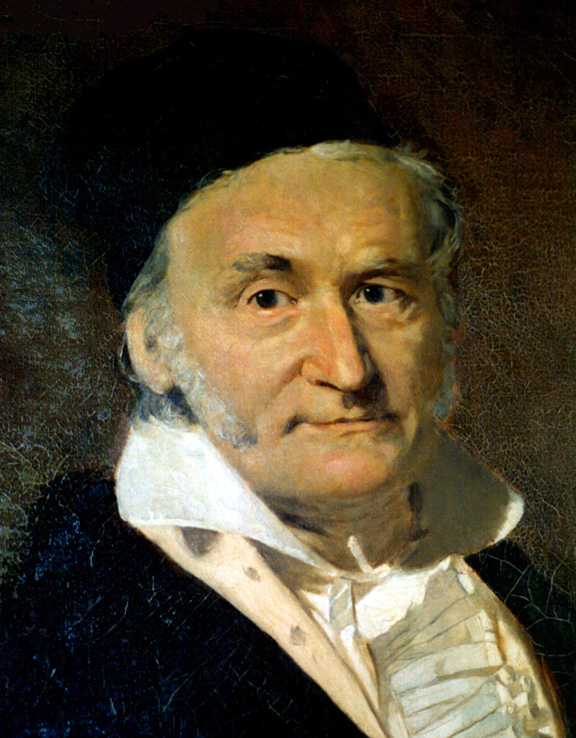
\includegraphics[width=0.25\linewidth]{gauss.jpg} \hfill 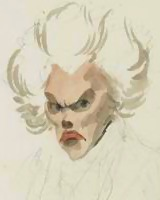
\includegraphics[width=0.258\linewidth]{lezhandr.jpg} \ \\\end{minipage} & Метод оценивания параметров эконометрической модели, состоящий в минимизации суммы квадратов расхождений между наблюдаемыми значениями зависимой переменной и значениями этой переменной, вычисленными для наблюдаемых значений независимых переменных по оценённой модели связи. \\
\hline
Обобщённый метод наименьших квадратов (GLS) &  
$$(X^T \Omega^{-1} X)^{-1}X^T \Omega^{-1} y$$
& 1934 & Alexander Aitken & \begin{minipage}[t]{\linewidth} \centering \ \\ 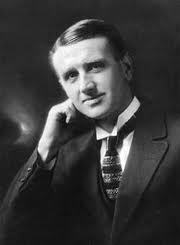
\includegraphics[width=0.25\linewidth]{alexander_craig_aitken_1_large.jpg} \\ \ \\\end{minipage} & Теоретическая процедура оценивания коэффициентов линейной модели регрессии в ситуации, когда случайные ошибки имеют разные дисперсии и коррелированы между собой, при этом предполагается,  что ковариационная матрица вектора ошибок невырождена и все ее элементы известны. \\
\hline
Взвешенный метод наименьших квадратов (WLS) &  $$(X^T \Omega^{-1} X)^{-1}  X^T \Omega^{-1}$$
\- $$\Omega~=~\diag(\sigma_1,\sigma_2, \ldots \sigma_n)$$ & 1934 & Alexander Aitken & \begin{minipage}[t]{\linewidth} \centering \ \\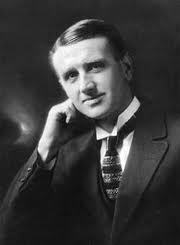
\includegraphics[width=0.25\linewidth]{alexander_craig_aitken_1_large.jpg}
\end{minipage} & Процедура, состоящая в минимизации определённым образом взвешенной суммы квадратов отклонений наблюдаемых значений зависиммой переменной от значений, вычисляемых по подбираемой модели связи. \\
\hline
Доступный обобщённый метод наименьших квадратов (FGLS) &  $$(X^T \hat{\Omega}^{-1} X)^{-1}X^T \hat{\Omega}^{-1} y$$ & 1934 & Alexander Aitken & \begin{minipage}[t]{\linewidth} \centering \ \\ 
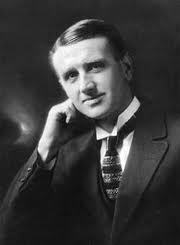
\includegraphics[width=0.25\linewidth]{alexander_craig_aitken_1_large.jpg} \hfill
\end{minipage} & Практически реализуемая процедура оценивания коэффициентов линейной модели регрессии в ситуации, когда случайные ошибки имеют разные дисперсии и коррелированы между собой, повторяющая процедуру обобщенного метода наисеньших квадратов, но импользующая оцененную ковариационную матрицу вектора ошибок. \\
\hline
Косвенный метод наименьших квадратов (ILS) & & \footnotesize{В}~1928 \footnotesize{начали заниматься проблемой инструментальных переменных}  & Philip Wright \newline Sewall Wright \newline \footnotesize{(отец и сын)}& 
\begin{minipage}[t]{\linewidth} \centering \ \\
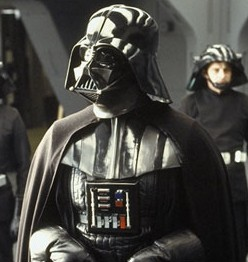
\includegraphics[width=0.25\linewidth]{Darth_Vader.jpg} \hfill
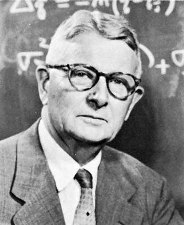
\includegraphics[width=0.22\linewidth]{Sewall_Wright.jpg}\ \\
\end{minipage} & Mетод получения оценок параметров $i-$го стохастического уравнения структурной формы через оценки наименьших квадратов коэффициентов уравнений приведенной формы. Метод применим в случае точной идентифицируемости $i-$го структурного уравнения.\\
\hline
Двухшаговый метод наименьших квадратов (2SLS) & $$(X^T Z (Z^T Z)^{-1} Z^T X)^{-1}$$\- $$X^T Z(Z^T Z)^{-1} Z^Ty $$ & 1953 \newline   1957 & Henri Theil \newline Robert Basmann & \begin{minipage}[t]{\linewidth} \centering \ \\
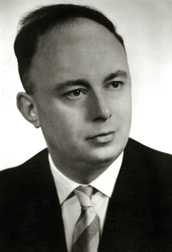
\includegraphics[width=0.24\linewidth]{apf1-08280t.jpg} \hfill 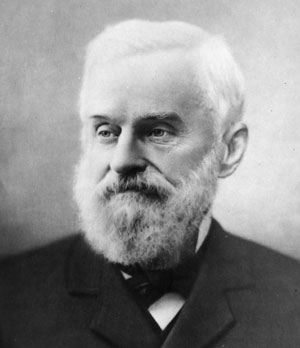
\includegraphics[width=0.3\linewidth]{AdonijahWelch.jpg}\ \\
\end{minipage} &  Метод оценивания коэффициентов уравнения структурной формы, состоящий в предварительной очистке стохастической объясняющей переменой от коррелированности с ошибкой в этом уравнении с использованием инструментальных переменных и в последующем оценивании уравнения, в котором исходная объясняющая переменная заменяется ее очищенным вариантом. \\
\hline
Трёхшаговый метод наименьших квадратов (3SLS) & $$(\hat Z^T(\hat \Lambda^{-1} \otimes I_g) \hat Z)^{-1}$$ \-
 $$\hat Z^T \newline(\hat \Lambda^{-1} \otimes I_g)y$$ & 1953 \newline   1957 &  Henri Theil \newline Robert Basmann &  
\begin{minipage}[t]{\linewidth} \centering \ \\
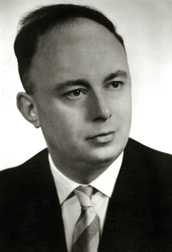
\includegraphics[width=0.24\linewidth]{apf1-08280t.jpg}\hfill 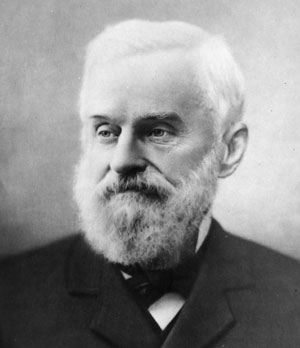
\includegraphics[width=0.3\linewidth]{AdonijahWelch.jpg}\ \\
\end{minipage}
 & Доступный обобщённый метод наименьших квадратов, применённый к системе одновременных уравнений. Принимает во внимание наличие коррелированности между ошибками в разных структурных уравнениях. \\
\hline

\end{tabular}
\caption{Разновидности МНК}
\end{table}
\end{document}



